% !TEX TS-program = pdflatex
\documentclass[border=5pt]{standalone}
\usepackage{tikz}
\usetikzlibrary{arrows.meta, positioning, shapes, fit,calc}
\begin{document}

% tikz version of 
% Experimental Modeling Framework
% see
% The modelling framework for experimental physics: Description, development, and applications
% by Dounas-Frazer, Dimitri R and Lewandowski, HJ
% European Journal of Physics, 2018
% doi 10.1088/1361-6404/aae3ce
% and
% https://jila.colorado.edu/lewandowski/research/experimental-modeling-framework-0
% https://jila.colorado.edu/sites/default/files/group_files/lewandowski/EMF.pdf

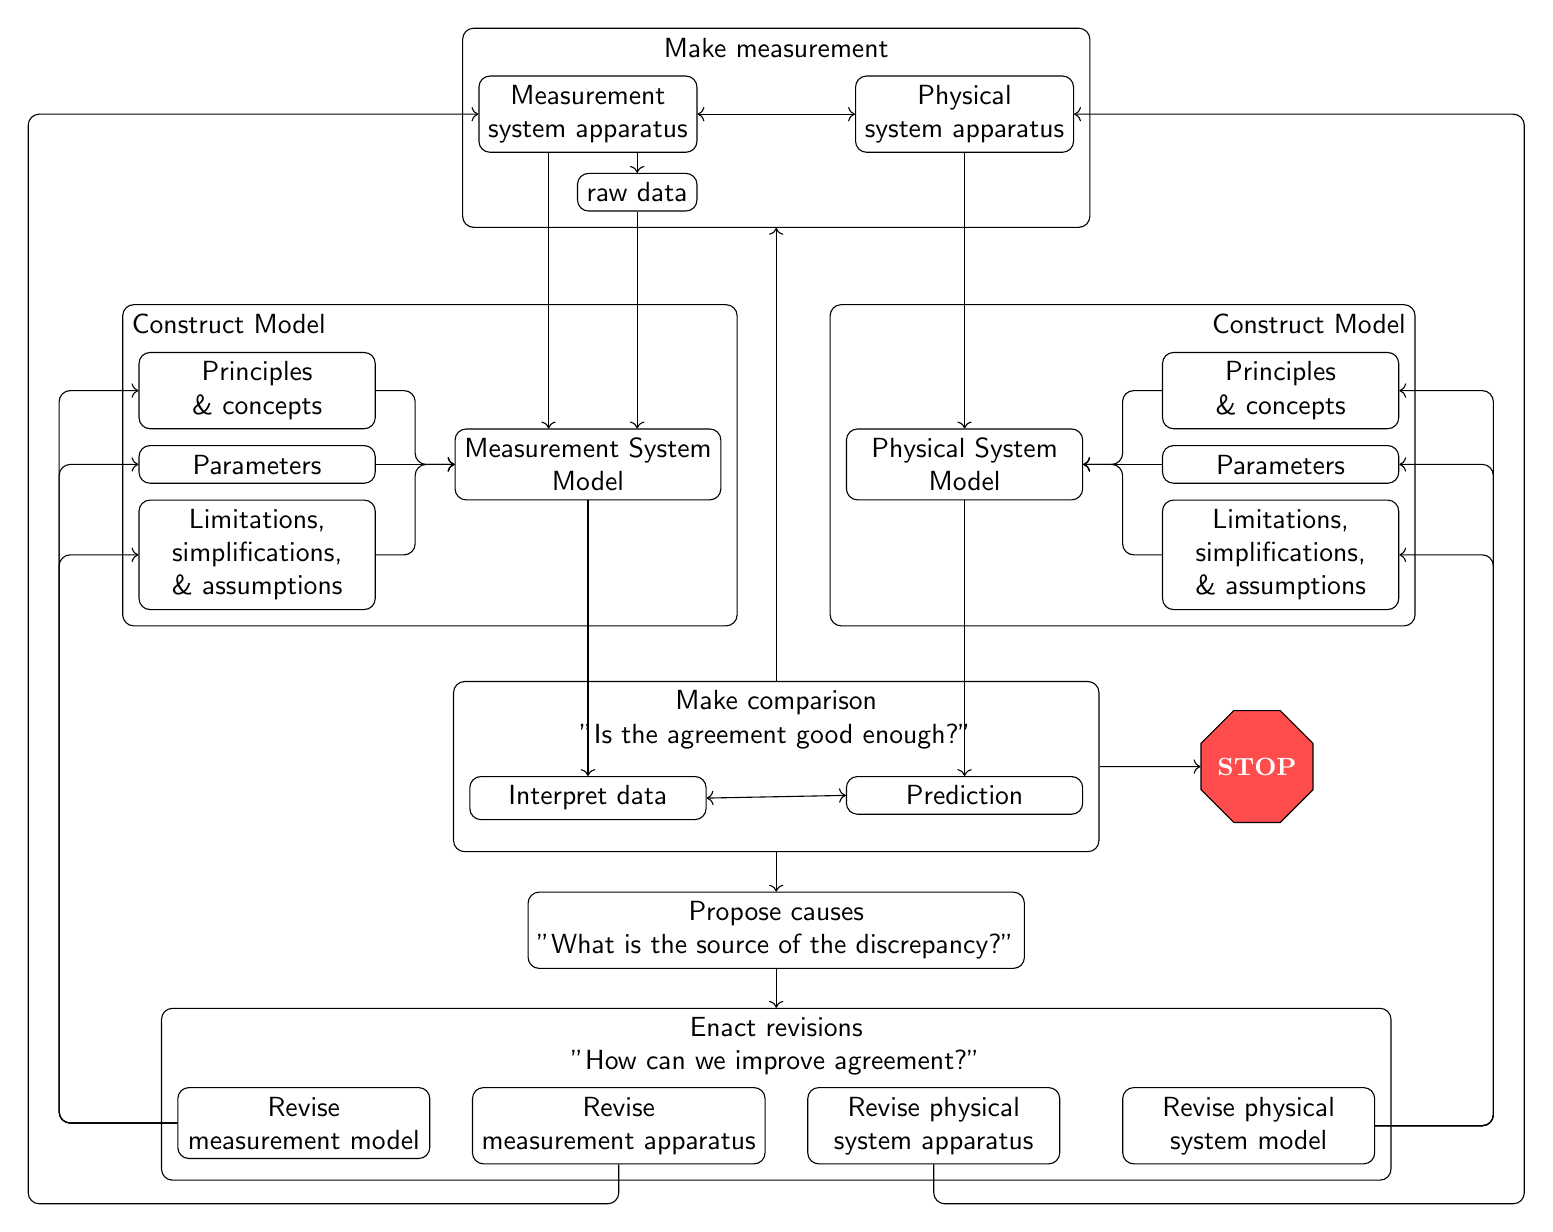
\begin{tikzpicture}[
  font=\sffamily,
  every node/.style={align=center},
  block/.style={draw, rounded corners},
]

% make Measurements
\node [block] (meas_app) {Measurement \\ system apparatus};
\node [block] (phys_app) [right=20mm of meas_app] {Physical \\ system apparatus};
\node [block] (raw_data) [below=5mm of meas_app, anchor=east] at (meas_app.east |- meas_app.south) {raw data};
\draw [<->] (meas_app.east) -- (phys_app.west);
\draw [<-] (raw_data.north) -- (raw_data.north |- meas_app.south);

\node (measure) [
          font=\bfseries, 
          fit=(meas_app) (phys_app) (raw_data),
          yshift=0.2cm, 
          inner ysep=0.4cm,inner xsep=0.2cm,
          draw,
          label={[label distance=-5mm]90:Make measurement}, 
          rounded corners] {};


% Construct Models

\node [block, minimum width=3cm, below=35mm of meas_app] (meas_model) {Measurement System \\ Model};

\node [block, minimum width=3cm, left=10mm of meas_model] (parametersM) {Parameters};
\node [block, minimum width=3cm] (principlesM) [above=2mm of parametersM] {Principles \\ \& concepts};
\node [block, minimum width=3cm] (limitationsM) [below=2mm of parametersM] {Limitations, \\ simplifications, \\ \& assumptions};

\draw[->, rounded corners] (parametersM.east) --  (meas_model.west);
\draw[->, rounded corners] (principlesM.east) -- ++(0.5,0 ) |-  (meas_model.west);
\draw[->, rounded corners] (limitationsM.east) --  ++(0.5,0 ) |-  (meas_model.west);


\node (meas_model_box) [
          font=\bfseries, 
          fit=(meas_model) (principlesM) (limitationsM) (parametersM),
          yshift=0.2cm, 
          inner ysep=0.4cm,inner xsep=0.2cm,
          draw,
        label={[anchor=north west]north west:Construct Model}, 
          rounded corners] {};


\draw[->] (raw_data.south) -- (raw_data.south |- meas_model.north);
\draw[->] ([xshift=-5mm]meas_app.south) -- ([xshift=-5mm]meas_app.south |- meas_model.north);


% the same but mirrored for the physical system
\node [block, minimum width=3cm, below=35mm of phys_app] (phys_model) {Physical System \\ Model};   
\node [block, minimum width=3cm, right=10mm of phys_model] (parametersP) {Parameters};
\node [block, minimum width=3cm] (principlesP) [above=2mm of parametersP] {Principles \\ \& concepts};
\node [block, minimum width=3cm] (limitationsP) [below=2mm of parametersP] {Limitations, \\ simplifications, \\ \& assumptions};

\draw[->, rounded corners] (parametersP.west) --  (phys_model.east);
\draw[->, rounded corners] (principlesP.west) -- ++(-0.5,0 ) |-  (phys_model.east);
\draw[->, rounded corners] (limitationsP.west) --  ++(-0.5,0 ) |-  (phys_model.east);


\node (phys_model_box) [
          font=\bfseries, 
          fit=(phys_model) (principlesP) (limitationsP) (parametersP),
          yshift=0.2cm, 
          inner ysep=0.4cm,inner xsep=0.2cm,
          draw,
        label={[anchor=north east]north east:Construct Model}, 
          rounded corners] {};


\draw[->] (phys_app.south) -- (phys_app.south |- phys_model.north);

% Make Comparisons
\node [block, minimum width=3cm, below=35mm of meas_model] (interpret) {Interpret data};
\node [block, minimum width=3cm, below=35mm of phys_model] (prediction) {Prediction};
\node (compare) [
          font=\bfseries, 
          fit=(interpret) (prediction),
          yshift=4mm, 
          inner ysep=8mm,inner xsep=0.2cm,
          draw,
        label={[anchor=north]Make comparison \\ "Is the agreement good enough?"}, 
          rounded corners] {};

\draw[->] (meas_model.south) -- (interpret.north);
\draw[->] (phys_model.south) -- (prediction.north);
\draw[<->] (interpret.east) -- (prediction.west);

% Propose Causes
\node [block, minimum width=3cm, below=5mm of compare] (propose) {Propose causes \\ "What is the source of the discrepancy?"};

\draw[->] (compare.south) -- (propose.north);
\draw[->] (compare.north) -- (measure.south);

% draw stop sign right of compare
\node[regular polygon, regular polygon sides=8, draw, fill=red!70, 
font=\bfseries\small, inner sep = 0mm, text=white] (stop) 
at ([xshift=20mm]compare.east) {STOP};

\draw[->] (compare.east) -- (stop.west);

% Enact Revisions
\node [block, minimum width=3.2cm] (revise1) [below=15mm of propose, xshift=-6cm] {Revise \\ measurement model};
\node [block, minimum width=3.2cm] (revise2) [below=15mm of propose, xshift=-2cm] {Revise \\ measurement apparatus};
\node [block, minimum width=3.2cm] (revise3) [below=15mm of propose, xshift=2cm] {Revise physical \\ system apparatus};
\node [block, minimum width=3.2cm] (revise4) [below=15mm of propose, xshift=6cm] {Revise  physical \\ system model};

\node (revise) [
          font=\bfseries, 
          fit=(revise1) (revise2) (revise3) (revise4),
          yshift=4mm, 
          inner ysep=6mm,inner xsep=0.2cm,
          draw,
        label={[anchor=north]Enact revisions \\ "How can we improve agreement?"}, 
          rounded corners] {};  

\draw[->] (propose.south) -- (revise.north);

\draw[->, rounded corners] (revise4.east) -- ++(1.5,0) |- (parametersP.east);
\draw[->, rounded corners] (revise4.east) -- ++(1.5,0) |- (principlesP.east);
\draw[->, rounded corners] (revise4.east) -- ++(1.5,0) |- (limitationsP.east);

\draw[->, rounded corners] (revise3.south) -- ++(0,-0.5) -- ++(7.5,0)  |- (phys_app.east);

\draw[->, rounded corners] (revise2.south) -- ++(0,-0.5) -- ++(-7.5,0)  |- (meas_app.west);

\draw[->, rounded corners] (revise1.west) -- ++(-1.5,0) |- (parametersM.west);
\draw[->, rounded corners] (revise1.west) -- ++(-1.5,0) |- (principlesM.west);
\draw[->, rounded corners] (revise1.west) -- ++(-1.5,0) |- (limitationsM.west);


\end{tikzpicture}
\end{document}
